\chapter{Unificando la WGAN y el WAE}\label{chap:WAE-WGAN}  % MARK: Unificando la WGAN y el WAE

En capítulos anteriores se explica que, tanto las WGANs como las WAEs aproximan una distribución real $\Prob_X$, además permiten aproximar las variedades, como también proyectar sobre ellas.
Por este motivo, en este trabajo se estima una distribución de imágenes $\Prob_X$ para tener acceso a un muestreo rápido de este, además, para que los baricentros sean naturales, se utiliza una estructura de AE para proyectar sobre la variedad de imágenes, siguiendo el trabajo de \cite{simon2020barycenters}.


Con respecto a la estimación de la distribución real y la aproximación de variedades, la WGAN realiza estas dos tareas bastante bien, gracias a su componente adversaria. Sin embargo, este no posee un codificador (que es necesario para poder proyectar sobre la variedad de imágenes). Por el otro lado, el WAE posee este codificador, pero no es tan bueno generando muestras de la distribución real o aproximando la variedad de imágenes. Cada una de estas estructuras cumplen bien con una de las tareas, pero no están diseñadas para cumplir con ambas.

\FM[inline]{Se podría agregar referencias de trabajos anteriores que tienen un AE adversario, que conectan ambos modelos, pero que no se ha visto una versión Wasserstein, que permite converjer en la top. débil}

Por esta razón, se propone un modelo que unifique a la WGAN y al WAE, de manera que se pueda estimar la distribución real y proyectar sobre la variedad de imágenes. A continuación se detalla la estructura de este modelo.

\section{Preparación del Conjunto de Datos}\label{ssec:preparacion-dataset}  % MARK: - Preparación del Conjunto de Datos

Para los experimentos, se utiliza el conjunto de datos $Quick, Draw!$, creada por Google \cite{jongejan2016quick}. Este conjunto de datos ha sido construido a través de un juego en línea, donde a los jugadores se les solicita dibujar objetos pertenecientes a una clase particular de objetos, en menos de 20 segundos. El conjunto de datos contiene 50 millones de dibujos en escala de grises divididos en cientos de tipos de clases.

Para la preparación del conjunto de datos, se ha desarrollado la librería \textit{Quick, Torch!} \cite{munoz2023quicktorch} para obtener fácilmente los datos utilizando la API de Google.
En los experimentos se utilizan específicamente las categorías ``Faces'' y ``Smiley Faces'', dado que poseen imágenes bastante similares. Sin embargo, en ambos conjuntos existen imágenes anómalas, además de que en la categoría ``Smiley Faces'' existe una mayor diversidad de imágenes. Por este motivo, es necesario realizar un tratamiento del conjunto de datos antes de utilizarlo. Un ejemplo de las imágenes de estas categorías se muestra en la Figura~\ref{fig:quick-draw-caras}.

\begin{figure}[htbp]
    \centering
    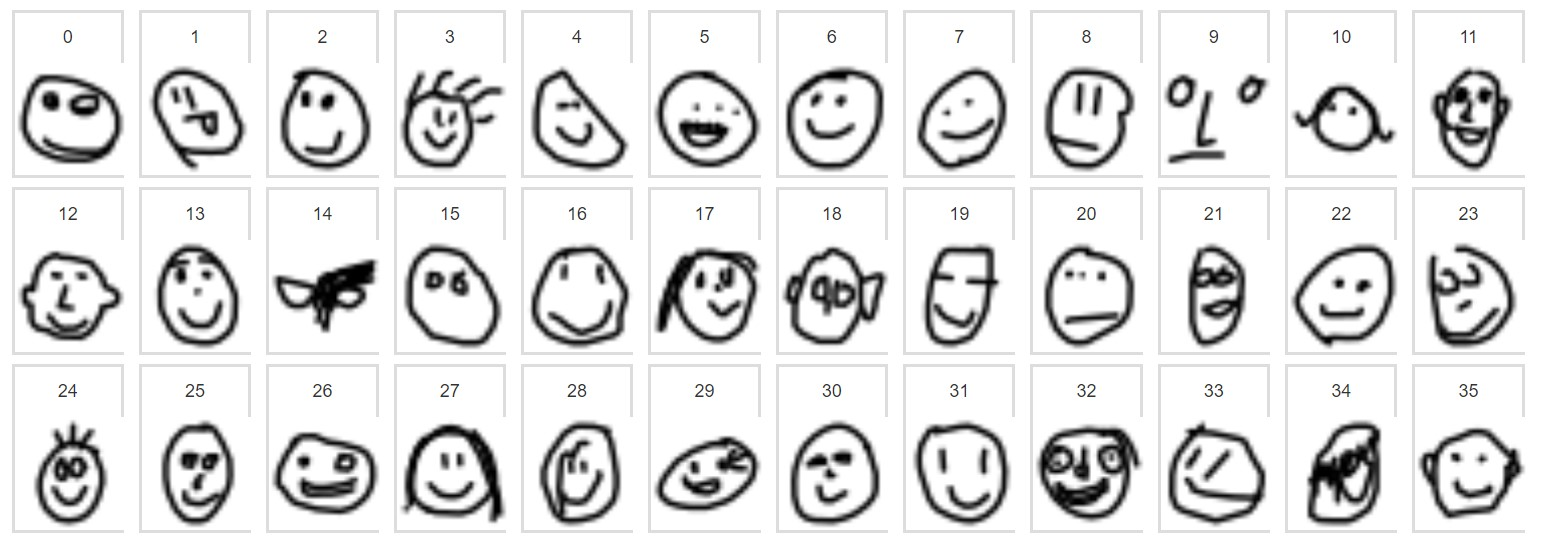
\includegraphics[width=0.75\textwidth]{img/quick-draw/caras.jpg}
    \caption{Ejemplo de imágenes de las categorías ``Faces'' y ``Smiley Faces''. Elaboración propia.}
    \label{fig:quick-draw-caras}
\end{figure}


Para la preparación del conjunto de datos, se han utilizado tanto técnicas de agrupamiento (también conocido como \textit{clustering}), como de reducción de dimensionalidad no lineal.
Iterativamente se reduce la dimensionalidad a través de la técnica llamada Aproximación y Proyección de Variedades Uniformes (UMAP, por sus siglas en inglés) \cite{mcinnes2018umap}, para después agrupar o limpiar los datos anómalos sobre dicha agrupación. Para agrupar los datos, se utilizan las técnicas de Agrupación Espacial de Aplicaciones con Ruido Basada en la Densidad (DBSCAN, por sus siglas en inglés) \cite{ester1996density}, o su variante jerárquica (HDBSCAN, por sus siglas en inglés) \cite{campello2013density};
mientras que para limpiar los datos anómalos, se usa el Factor Atípico Local (LOF, por sus siglas en inglés) \cite{breunig2000lof}. Después del tratamiento, en el conjunto de datos quedan $230$K imágenes en total. Las técnicas de agrupación y limpieza fueron utilizadas mediante la librería de \textit{scikit-learn} \cite{sklearn}.

A continuación se ilustran algunas imágenes en las que se utilizan las técnicas mencionadas.
En la Figura~\ref{fig:umap} se puede observar la proyección UMAP en dos dimensiones del conjunto de datos, donde claramente se notan dos agrupaciones. En la Figura~\ref*{fig:umap-clusterizado} se presentan las agrupaciones utilizando DBSCAN. Por último, en la Figura~\ref*{fig:umap-clusters} se presentan las imágenes correspondientes a cada etiqueta de la Figura~\ref*{fig:label2}. Se puede apreciar que en estas figuras se observa una tendencia clara en la forma en que se agrupan las imágenes.

\begin{figure}[H]
    \centering
    \begin{subfigure}[b]{0.45\textwidth}
        \centering
        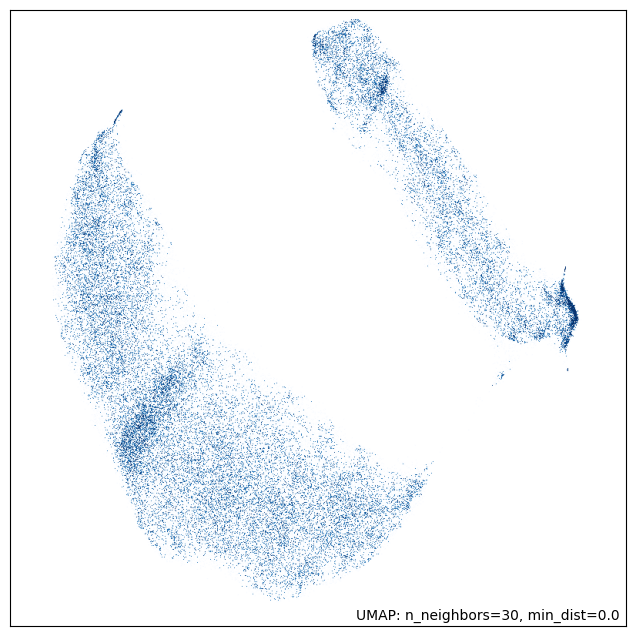
\includegraphics[height=6cm]{img/cleaning-data/umap.png}
        \caption{Proyección UMAP del conjunto de datos.}
        \label{fig:umap}
    \end{subfigure}
    \hfill
    \begin{subfigure}[b]{0.45\textwidth}
        \centering
        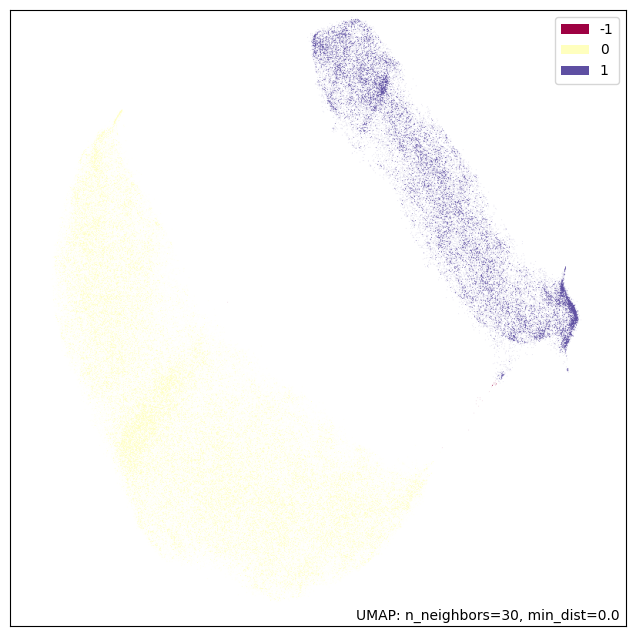
\includegraphics[height=6cm]{img/cleaning-data/umap-clusterizado.png}
        \caption{Proyección UMAP agrupada.}
        \label{fig:umap-clusterizado}
    \end{subfigure}
    \caption{Visualización de la proyección UMAP y su agrupación.}
    \label{fig:umap-example}
\end{figure}

\begin{figure}[H]
    \centering
    \begin{subfigure}[b]{0.45\textwidth}
        \centering
        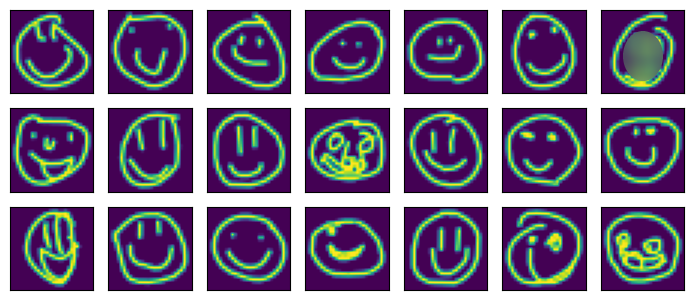
\includegraphics[width=\textwidth]{img/cleaning-data/label1.png}
        \caption{Imágenes de la etiqueta 0.}
        \label{fig:label1}
    \end{subfigure}
    \begin{subfigure}[b]{0.45\textwidth}
        \centering
        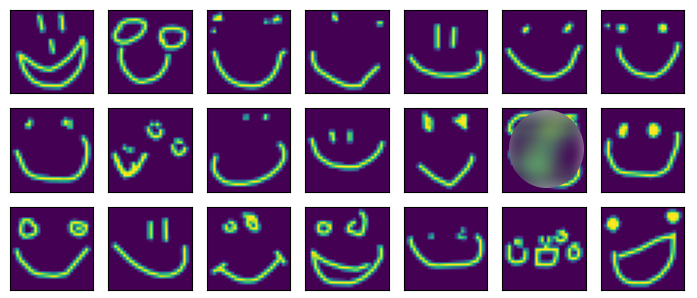
\includegraphics[width=\textwidth]{img/cleaning-data/label2.png}
        \caption{Imágenes de la etiqueta 1.}
        \label{fig:label2}
    \end{subfigure}
    \begin{subfigure}[b]{0.45\textwidth}
        \centering
        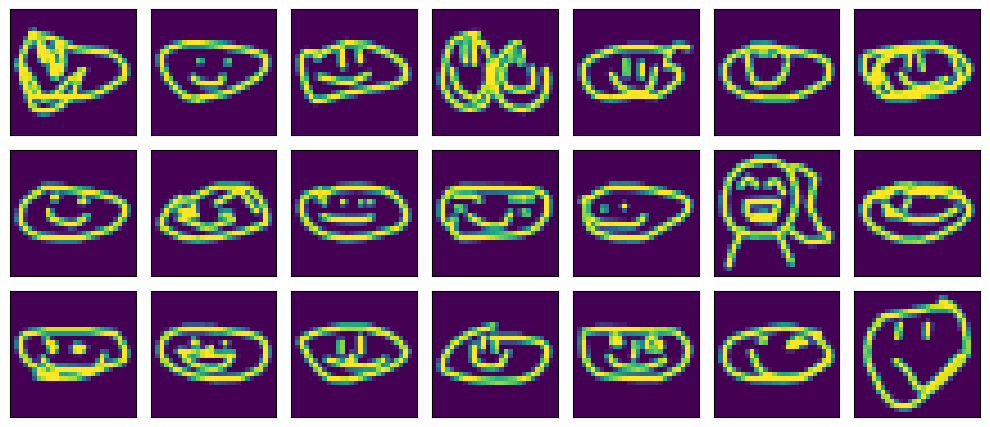
\includegraphics[width=\textwidth]{img/cleaning-data/outliers.png}
        \caption{Datos anómalos.}
        \label{fig:outliers}
    \end{subfigure}
    \caption{Imágenes correspondiente a los etiquetados en la Figura~\ref{fig:umap-clusterizado}.}
    \label{fig:umap-clusters}
\end{figure}

\FM[inline]{Finalmente, a las imagenes seleccionadas, se les realiza las siguientes transformaciones: ...}

Se redimensionan las imágenes de $28\times28$ a $32\times32$ píxeles y se normalizan para mejorar el entrenamiento de las redes neuronales. Se realizan diversas técnicas de aumento de datos (también conocido como \textit{data augmentation}), tales como: volteo horizontal aleatorio (o \textit{random horizontal flip}) con una probabilidad del $0.5$; alejamiento aleatorio (o \textit{random zoom out}) con una probabilidad del $0.3$ con un aumento que distribuye como una uniforme de rango $[1; 1.25]$ y rotación aleatoria (o \textit{random rotation}) con un ángulo aleatorio entre $[-10, 10]$.

\RED[inline]{¿Se podría dejar el párrafo anterior como una enumeración mejor?}

\section{Deducción de la arquitectura}\label{sec:deduccion-arquitectura-wae-wgan}  % MARK: - Deducción de la arquitectura

Como se menciona en los capítulos anteriores, la WGAN y el WAE tienen tareas similares: buscan minimizar una estimación de la distancia de Wasserstein entre una distribución de referencia $\Prob_X$ y una distribución generadora $\Prob_G$. En particular, la WGAN lo realiza utilizando la $1$-distancia de Wasserstein, mientras que el WAE lo puede hacer con cualquier distancia definida a través de la función de costo $c$.

Por este motivo, la deducción del algoritmo es simple: dejar que la WGAN entrene la generadora y la función crítica, de manera que la generadora ya esté bastante cerca de la distribución real. Luego, se puede utilizar la generadora de la WGAN como decodificadora del WAE, y entrenar esta última arquitectura (donde la generadora ya está más cerca de parecerse a la distribución real) para que el codificador sea capaz de proyectar sobre la variedad de imágenes. Es importante que la función de costo del WAE sea $c(x, y) = |x - y|$ para que se esté calculando la $1$-distancia de Wasserstein, y la distribución de la decodificadora converja en la misma topología que la WGAN.


Por este motivo, el algoritmo propuesto es el siguiente:

\begin{algorithm}[H]
    \caption{Entrenamiento de una WAE-WGAN, elaboración propia}\label{alg:WAE-WGAN}
    \begin{algorithmic}[1]
        \Require Tamaño del batch $N$, número de iteraciones para el discriminador $N_d$ y los parámetros de penalización $\lambda_{\mathrm{WGAN}}$ y $\lambda_{\mathrm{WAE}}$.
        \State Inicializar los parámetros de la generadora $G_\theta$ y la función crítica $f_\omega$.
        \While{$\theta$ no ha convergido}
        \State // {Entrenamiento de la función crítica}
        \For{$t=1,\ldots,N_d$}
        \State Muestrear $\{x_i\}_{i=1}^{N} \sim \Prob_X$ desde el conjunto de entrenamiento.
        \State Muestrear $\{z_i\}_{i=1}^{N} \sim \Prob_Z$ desde el espacio latente.
        \State $\tilde x \gets (G_\theta(z_i))_{i=1}^{N}$.
        \State $\cL_{\mathrm{critic}} \gets
            \frac{1}{N} \sum_{i=1}^{N} f_{\omega}(\tilde x_i) - \frac{1}{N} \sum_{i=1}^{N} f_{\omega}(x_i) + \lambda_{\mathrm{WGAN}} \cdot \Call{penalty}{\omega, x, \tilde x}$
        \State Actualizar $f_{\omega}$ por medio de descenso de gradiente en $\pdv{\omega} \cL_{\mathrm{critic}}$.
        \EndFor
        \State // {Entrenamiento de la generadora por parte de la WGAN}
        \State Muestrear $\{z_i\}_{i=1}^{N} \sim \Prob_Z$ desde el espacio latente.
        \State $\cL_{\mathrm{gen}} \gets - \frac{1}{N}\sum_{i=1}^{N} f_\omega(G_\theta(z_i))$
        \State Actualizar $G_\theta$ por medio de descenso de gradiente en $\pdv{\theta} \cL_{\mathrm{gen}}$.
        \State // {Entrenamiento de la WAE}
        \State Muestrear $\{z_i\}_{i=1}^{N} \sim \Prob_Z$ desde el espacio latente.
        \State Muestrear $\tilde z_i \sim \ProbQ_\varphi(\dd z \mid x_i)$ para $i=1\dots N$.
        \State Obtener $\tilde x_i \gets G_\theta(\tilde z_i)$ para $i=1\dots N$.
        \State $\cL_{\mathrm{AE}} \gets \frac{1}{N}\sum_{i=1}^{N} |x_i - \tilde x_i| + \lambda_{\mathrm{WAE}} \cdot \Call{similarity}{z, \tilde z}$
        \State Actualizar $\ProbQ_\varphi$ y $G_\theta$ por medio de descenso de gradiente en $\pdv{\varphi} \cL_{\mathrm{AE}}$ y $\pdv{\theta} \cL_{\mathrm{AE}}$.
        \EndWhile
    \end{algorithmic}
\end{algorithm}

Donde la función $\Call{penalty}{\omega, x, \tilde x}$ es alguna penalización para asegurar que $f_\omega\in \Lip_1(\cX)$, y $\Call{similarity}{z, \tilde z}$ es alguna función de similitud entre densidades (como MMD o alguna otra divergencia o distancia) entre las distribuciones $\Prob_Z$ y $\ProbQ_{Z, \varphi} \eqdef \int_{\cX} \ProbQ_\varphi(\bullet \mid x) \Prob_X(\dx)$. Definir el algoritmo de esta manera permite tener una mayor generalidad a la hora de utilizarlo, y poder experimentar con distintas funciones de penalización y similitud.

Notar que el Algoritmo~\ref{alg:WAE-WGAN} realiza alternadamente tres procesos. Primero, un entrenamiento de la función crítica. Luego, un entrenamiento de la generadora, utilizando una estimación de la distancia de Wasserstein en su versión de la WGAN. Finalmente, un entrenamiento del WAE, el que entrena simultáneamente a la codificadora y generadora. Para estos efectos, la generadora se entrena con el gradiente de la distancia de Wasserstein por ambos algoritmos en una sola iteración.


Además, cuando la función crítica y la decodificadora alcanzan un máximo y mínimo aceptable, respectivamente, entonces la evaluación de estas redes en las funciones de pérdida provee una estimación de la distancia de Wasserstein para ambos casos. Esto resulta útil para monitorear el entrenamiento de la red.

\subsubsection{Implementación}\label{sssec:wae-wgan-implementacion}  % MARK: - Implementación


El Algoritmo~\ref{alg:WAE-WGAN} se implementa utilizando la librería de \textit{PyTorch} \cite{paszke2019pytorch} a través de las redes neuronales convolucionales (CNN por sus siglas en inglés) [CITA], siguiendo la estrategia de ResNet \cite{he2016deep}. La red neuronal se entrena en tres variedades de imágenes diferentes, las cuales han sido obtenidas siguiendo los pasos explicados en la Sección~\ref{ssec:preparacion-dataset}. Algunas muestras de estas variedades se presentan en la Figura~\ref{fig:variedades-imagenes}. Se separa el conjunto de datos en un conjunto de entrenamiento y otro de validación, con un $95\%$ y $5\%$ de las imágenes, respectivamente.

\begin{figure}[H]
    \begin{subfigure}[b]{0.32\textwidth}
        \centering
        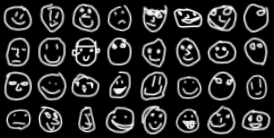
\includegraphics[width=\textwidth]{img/cluster/label1.png}
        \caption{1era variedad de imágenes.}
        \label{fig:label1-manifold}
    \end{subfigure}
    \hfill
    \begin{subfigure}[b]{0.32\textwidth}
        \centering
        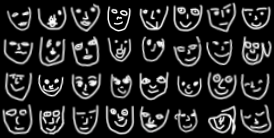
\includegraphics[width=\textwidth]{img/cluster/label2.png}
        \caption{2da variedad de imágenes.}
        \label{fig:label2-manifold}
    \end{subfigure}
    \hfill
    \begin{subfigure}[b]{0.32\textwidth}
        \centering
        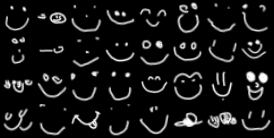
\includegraphics[width=\textwidth]{img/cluster/label3.png}
        \caption{3era variedad de imágenes.}
        \label{fig:label3-manifold}
    \end{subfigure}
    \caption{Variedades de imágenes utilizadas en los experimentos.}
    \label{fig:variedades-imagenes}
\end{figure}

A lo largo del entrenamiento se han registrado las estimaciones de la distancia de Wasserstein para la WGAN y el WAE, sobre el conjunto de validación para analizar la convergencia. En la Figura~\ref{fig:wass-dist} se presentan dichas estimaciones. Se puede observar que ambas estimaciones disminuyen a lo largo del entrenamiento, lo que corrobora que el algoritmo propuesto es estable, y además, indica que las redes están aprendiendo a aproximar la distancia de Wasserstein correctamente.
% , lo que indica que las redes están aprendiendo a aproximar la distancia de Wasserstein correctamente, además de que corrobora que el algoritmo propuesto es estable.

\begin{figure}[H]
    \begin{subfigure}[b]{0.8\textwidth}
        \centering
        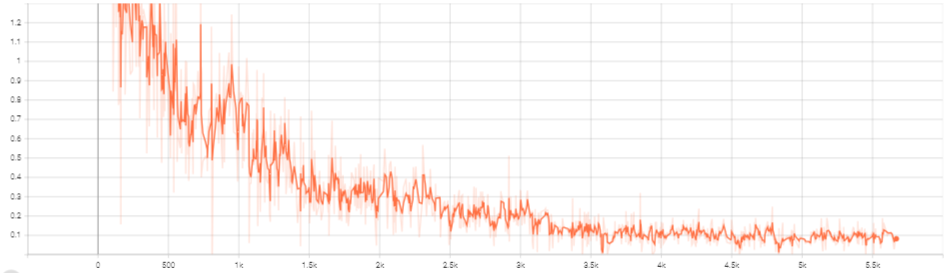
\includegraphics[width=\textwidth]{img/wgan-wae/wass-dist-wgan.png}
        \caption{Estimación de la distancia de Wasserstein para la WGAN.}
        \label{fig:wass-dist-wgan}
    \end{subfigure}
    % \hfill
    \begin{subfigure}[b]{0.8\textwidth}
        \centering
        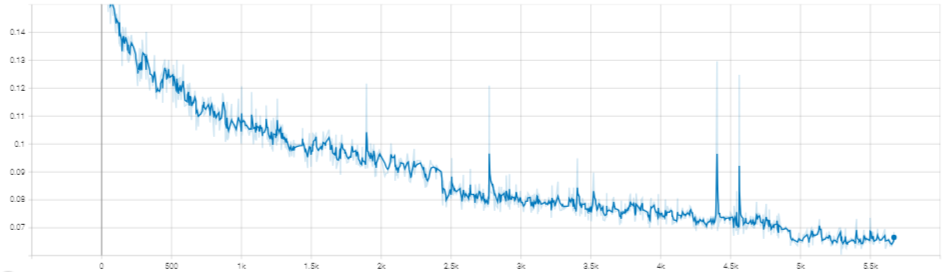
\includegraphics[width=\textwidth]{img/wgan-wae/wass-dist-wae.png}
        \caption{Estimación de la distancia de Wasserstein para el WAE.}
        \label{fig:wass-dist-wae}
    \end{subfigure}
    \caption{Estimación de la distancia de Wasserstein para la WGAN y el WAE.}
    \label{fig:wass-dist}
\end{figure}

Para validar que las redes generativas están aprendiendo a reconstruir y generar imágenes de calidad,
se presentan en la Figura~\ref{fig:generacion-imagenes} las imágenes reales, las decodificadas y las generadas por la WAE-WGAN.

\begin{figure}[H]
    % Primera variedad
    \begin{subfigure}[b]{0.32\textwidth}
        \centering
        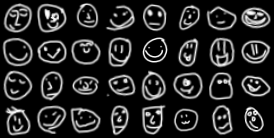
\includegraphics[width=\textwidth]{img/wgan-wae/real1.png}
        \caption{Img. reales.}
        \label{fig:real1}
    \end{subfigure}
    \hfill
    \begin{subfigure}[b]{0.32\textwidth}
        \centering
        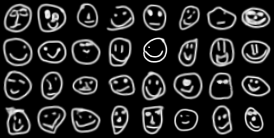
\includegraphics[width=\textwidth]{img/wgan-wae/decoded1.png}
        \caption{Img. decodificadas.}
        \label{fig:decoded1}
    \end{subfigure}
    \hfill
    \begin{subfigure}[b]{0.32\textwidth}
        \centering
        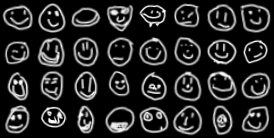
\includegraphics[width=\textwidth]{img/wgan-wae/gen1.png}
        \caption{Img. generadas.}
        \label{fig:gen1}
    \end{subfigure}
    % Segunda variedad
    \begin{subfigure}[b]{0.32\textwidth}
        \centering
        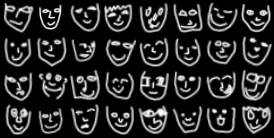
\includegraphics[width=\textwidth]{img/wgan-wae/real2.png}
        \caption{Img. reales.}
        \label{fig:real2}
    \end{subfigure}
    \hfill
    \begin{subfigure}[b]{0.32\textwidth}
        \centering
        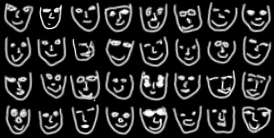
\includegraphics[width=\textwidth]{img/wgan-wae/decoded2.png}
        \caption{Img. decodificadas.}
        \label{fig:decoded2}
    \end{subfigure}
    \hfill
    \begin{subfigure}[b]{0.32\textwidth}
        \centering
        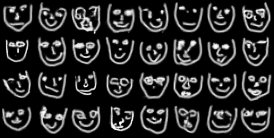
\includegraphics[width=\textwidth]{img/wgan-wae/gen2.png}
        \caption{Img. generadas.}
        \label{fig:gen2}
    \end{subfigure}
    % Tercera variedad
    \begin{subfigure}[b]{0.32\textwidth}
        \centering
        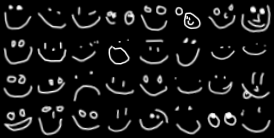
\includegraphics[width=\textwidth]{img/wgan-wae/real3.png}
        \caption{Img. reales.}
        \label{fig:real3}
    \end{subfigure}
    \hfill
    \begin{subfigure}[b]{0.32\textwidth}
        \centering
        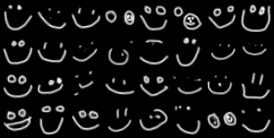
\includegraphics[width=\textwidth]{img/wgan-wae/decoded3.png}
        \caption{Img. decodificadas.}
        \label{fig:decoded3}
    \end{subfigure}
    \hfill
    \begin{subfigure}[b]{0.32\textwidth}
        \centering
        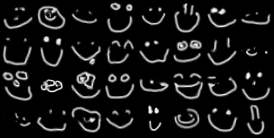
\includegraphics[width=\textwidth]{img/wgan-wae/gen3.png}
        \caption{Img. generadas.}
        \label{fig:gen3}
    \end{subfigure}
    \caption{Imágenes reales, decodificadas y generadas por la WGAN y el WAE en las tres variedades de imágenes. Cada fila corresponde a una variedad de imágenes.}
    \label{fig:generacion-imagenes}
\end{figure}

Se puede observar que las imágenes generadas por la WAE-WGAN son bastante similares a las imágenes reales, lo que indica que las redes están aprendiendo a aproximar la distribución real. Además, las imágenes decodificadas por el WAE son bastante similares a las imágenes originales, lo que muestra que la red está aprendiendo a proyectar sobre la variedad de imágenes simultáneamente.



% \section{Detalles de la implementación}\label{sec:detalles-implementacion}  % MARK: - Detalles de la implementación


% \subsection{WGAN con Gradiente Penalizado Generalizado}\label{ssec:wgan-ggp}  % MARK: - WGAN con Gradiente Penalizado Generalizado

% Como función de penalización para la función crítica, se desarrolla una forma novedosa de penalizar el gradiente, de manera que tenga mayor estabilidad. La idea es obtener un intermedio de una WGAN con penalización Lipschitz (WGAN-LP) \cite{zhou2018lp} y una WGAN con gradiente penalizado (WGAN-GP) \cite{gulrajani2017improved}.

% Dado los parámetros de penalización $\lambda_{GP} \geq 0$ y $\lambda_{LP} \geq 0$, se define la penalización como:
% \begin{align*}
%      & \lambda_{\mathrm{LP}} \Exp_{\hat x \sim \tau} \Big[\big(||\nabla_{\hat x} f_{\omega}(\hat x)||_2 - 1\big)_{+}^2\Big]
%     + \lambda_{\mathrm{GP}} \Exp_{\hat x \sim \tau} \Big[\big( - (||\nabla_{\hat x} f_{\omega}(\hat x)||_2 - 1)\big)_{+}^2\Big] \\
%      & =  \lambda_{\mathrm{LP}} \Exp_{\hat x \sim \tau} \Big[\big(||\nabla_{\hat x} f_{\omega}(\hat x)||_2 - 1\big)_{+}^2\Big]
%     + \lambda_{\mathrm{GP}} \Exp_{\hat x \sim \tau} \Big[\big( ||\nabla_{\hat x} f_{\omega}(\hat x)||_2 - 1 \big)_{-}^2\Big],
% \end{align*}
% donde $(x)_{+} \eqdef \max(0, x)$, $(x)_{-} \eqdef -\min(0, x)$ y se usa el hecho de que $(-x)_{+} = (x)_{-}$. De esta manera, la expresión de la ecuación anterior se puede reescribir de la siguiente forma:
% \begin{equation}
%     \lambda_{\mathrm{LP}} \Exp_{\hat x \sim \tau} [\mathrm{LeakyReLU}_{\rho}(||\nabla_{\hat x} f_{\omega}(\hat x)||_2 - 1)^2],
% \end{equation}
% con $\rho = \sqrt{\frac{\lambda_{GP}}{\lambda_{LP}}}$ y recordando que
% \begin{equation}
%     \mathrm{LeakyReLU}_{\rho} (x) \eqdef \begin{cases}
%         \rho x & \text{si } x < 0,    \\
%         x      & \text{si } x \geq 0.
%     \end{cases}
% \end{equation}

% La razón de por qué es una generalización, es porque si se toma $\lambda_{\mathrm{GP}} = \lambda_{\mathrm{LP}}$ entonces se recupera la penalización de la WGAN-GP, y si se toma $\lambda_{\mathrm{GP}} = 0$ entonces se recupera la penalización de la WGAN-LP. De esta manera, se puede tener un control más fino de la penalización del gradiente. Por este motivo, a las WGANs que utilizan esta función de penalización, se les llamará \textit{WGAN con gradiente penalizado generalizado} (WGAN-GGP por sus siglas en inglés).

% En los experimentos, se utiliza $\lambda_{\mathrm{LP}} = 10$ y $\lambda_{\mathrm{GP}} = 0.1$ para tener una penalización más fuerte cuando la norma del gradiente es mayor a $1$, pero muy baja cuando sea menor a 1. La diferencia entre la penalización mayor y menor es de 100:1, por lo que esta última, funciona como un incentivo, ayudando a la función $f_\omega$ a acercarse a la frontera de las funciones $1$-Lipschitz.

% \FM[inline]{Incluir el algoritmo para el cálculo de la penalización}

% \subsection{Arquitectura de la Red}\label{ssec:arquitectura-red}  % MARK: - Arquitectura de la Red

% \FM[inline]{Cada vez que utilice pytorch lo nombro y lo cito (para que quede más claro)}

% Las redes neuronales son implementadas utilizando la librería de \textit{PyTorch} \cite{paszke2019pytorch}. Se utilizan redes neuronales convolucionales (CNN por sus siglas en inglés) siguiendo la estrategia de ResNet \cite{he2016deep} para la codificadora $\ProbQ_\varphi$, la generadora $G_\theta$ y la función crítica $f_\omega$.


% \FM[inline]{Ojalá incluir alguna imagen que ilustre la arquitectura}
% \FM[inline]{Aquí incluir la arquitectura de la red}

% \section{Resultados}\label{sec:resultados-wae-wgan}  % MARK: - Resultados

% \FM[inline]{Incluir las imágenes de las diferencias entre las categorías de caras y caras felices}
% \FM[inline]{Incluir fotos de la variedad y clusterización}
% \FM[inline]{Mostrar gráficos de las funciones de pérdida y de la distancia de Wasserstein}
% \FM[inline]{Incluir gráficos de las imágenes generadas y reconstruidas}

\section{Conclusiones}\label{sec:conclusiones-wae-wgan}  % MARK: - Conclusiones


A vista de los resultados, se puede concluir que la WAE-WGAN es capaz de generar imágenes de calidad y a la vez entrenar un codificador, de manera que se pueda proyectar sobre la variedad de imágenes. Además, se destaca que la WAE-WGAN es capaz de aproximar la distancia de Wasserstein, lo que indica que la red está aprendiendo a aproximar la distribución real.

